\chapter{Ανίχνευση προσώπων με τον αλγόριθμο Viola-Jones}\label{ch:violajones}

This chapter concentrates on Ganeti. We will discuss the architecture of Ganeti,
and we will analyze in details its most basic parts and how they interact with
each other. We will try to provide small documentation to familiarize the reader
with this tool, avoiding presenting superfluous information. Summing up, the
objective for the reader is at the end of this chapter to have a comprehensive
view of Ganeti and its basic structure.

\section{Overview}

Ganeti is a software tool to manage computer clusters, and also assumes the
management task of the virtual instances of the cluster. Is is being
developed by Google and is an Open Source Project since 2007. It is build on top
of existing virtualization technologies, such as XEN or KVM hypervisors, and
other open source software. It also uses LVM for disk management, optionally
DRBD for disk replication across physical hosts, and other disk templates such
as RBD, external shared storage providers and more.

Ganeti uses a daemon-based model. Each daemon deals with specific tasks that the
cluster has to face, and communicates with other daemons using various
protocols, mainly HTTP based, and custom ones like LUXI. Many of those daemons
are written in Haskell, but most of the project's code is in Python. Ganeti is
actually a wrapper around hypervisors. Once installed, the tool will take over
the management part of virtual instances. It also makes it convenient for system
administrators to setup and handle clusters of physical nodes.

Some of the main features that Ganeti provides, and controls are the following:

\begin{itemize}
  \item Cluster management of physical nodes.
  \item Support for XEN virtualization.
  \item Support for KVM virtualization.
  \item Support for virtual console to control instances ,e.g, VNC.
  \item Support for live instance migration.
  \item Support for virtio or emulated devices.
  \item Disk management: plain LVM volumes, files, Across-the-network RAID1
        (using DRBD) for quick recovery in case of physical system failure.
  \item Export/import mechanisms for backup purposes or migration between
        cluster.
  \item Fast and simple recovery after physical failures using commodity
        hardware.
\end{itemize}

\section{Terminology}

In this section, we provide a small introduction of the most basic Ganeti terms,
in order to facilitate the reader in the rest of the document. In
Figure~\ref{fig:gnt_abst}, we present an abstract Ganeti architecture, which will
help us to briefly explain those terms.

\begin{figure}[htbp]
  \begin{center}
    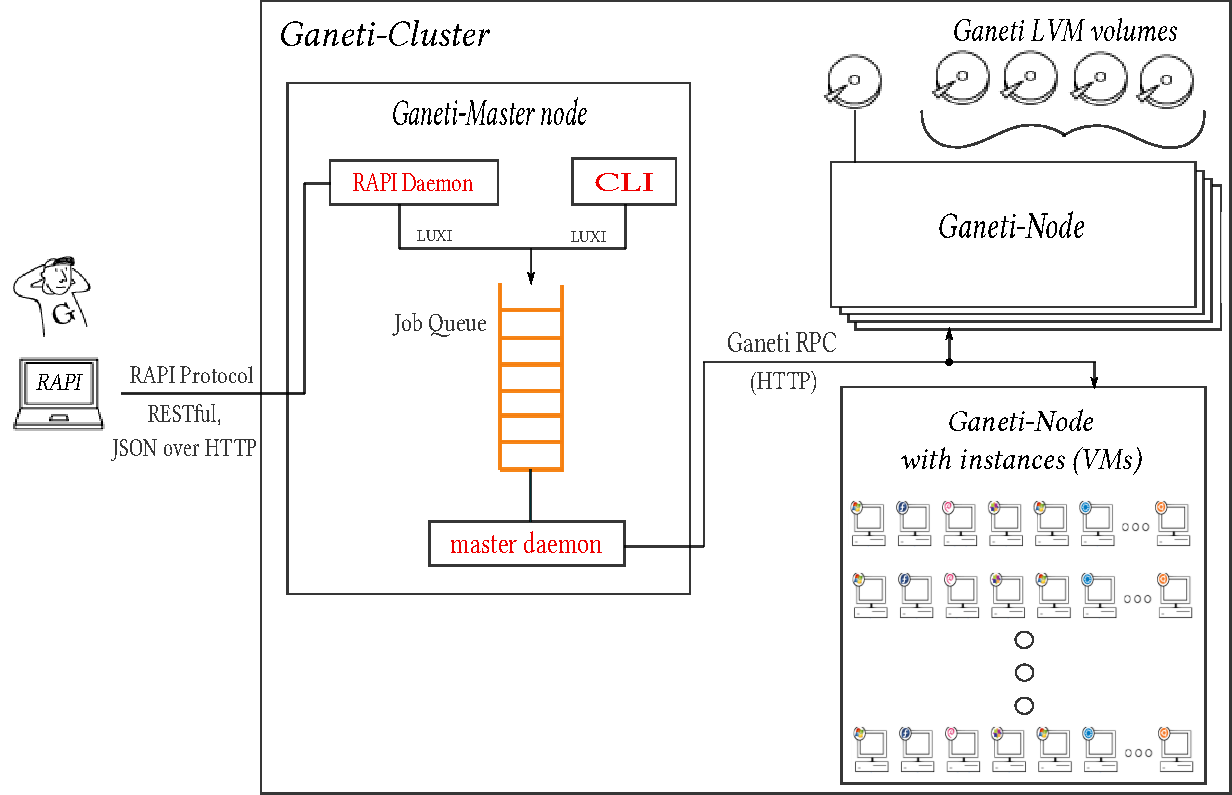
\includegraphics[width=1.0\maxwidth]{../figures/ganeti_abst_arch.pdf}
    \caption{Ganeti base components, version 2.7.2\label{fig:gnt_abst}}
   \end{center}
\end{figure}

\begin{description}
  \item[Cluster] \hfill \\
    A set of computers (nodes) working together to provide a coherent, reliable,
    scalable, highly-available virtualization service under a single domain.
  \item[Node] \hfill \\
    A physical machine which corresponds to the basic cluster infrastructure. If
    they host no instances, nodes can be added and removed at will from the
    cluster. They do not have to be fault-tolerant in order to achieve
    high availability for the instances they host. The loss of a single node,
    in a HA cluster, will not cause disk data loss for any of the instances it
    hosts.

    A node belonging to a cluster can serve different roles; VM-hosting and/or
    Administrative roles, which will be explained later in this document.
    Independently of its role, nodes can be in different statuses like online,
    drained or offline. Depending on the role they serve, each node will run a
    set of daemons:

    \begin{itemize}
      \item ganeti-masterd
      \item ganeti-noded
      \item ganeti-rapid
      \item ganeti-confd
    \end{itemize}
  \item[Instance] \hfill \\
    A virtual machine that runs on a cluster. Instances in Ganeti are
    highly-available entities, that can also become fault-tolerant depending on
    the disk template they use, e.g., DRBD. An instance has various parameters
    which can be modified either at instance level or at cluster level via
    cluster default parameters. Those parameters can be classified in three
    main categories: hypervisor related parameters, called \texttt{hvparams},
    general parameters, called \texttt{beparams}, and network interface
    parameters, called \texttt{nics}.
  \item[Disk Template] \hfill \\
    The layout disk type for the instance. Instances in Ganeti see the same
    virtual drive in all cases, but the node-level configuration varies between
    them. The available storage templates are the following:
    \begin{description}
      \item[diskless] \hfill \\
        This creates an instance with no disks. Useful for testing purposes, or
        other special cases.
      \item[file] \hfill \\
        Disk devices will be regular plain files. No redundancy is provided.
      \item[sharedfile] \hfill \\
        Disk devices will be regular plain files under a shared directory. This
        option allows live migration and failover of instances.
      \item[plain] \hfill \\
        Disk devices will be LVM volumes.
      \item[drbd] \hfill \\
        Disk devices will be drbd on top of LVM volumes, compatible with DRBD
        versions 8.x.
      \item[rbd] \hfill \\
        Disk devices will be rbd volumes, short for RADOS block device, residing
        inside a RADOS cluster.
      \item[blockdev] \hfill \\
        Pre-existent block devices will be used as backend for its disks.
      \item[ext] \hfill \\
        The instance will use an external storage provider as disk backend,
        through the ExtStorage Interface, using ExtStorage providers.
    \end{description}
  \item[\emph{Primary} and \emph{Secondary} concepts] \hfill \\
    An instance has a primary node, and depending on the disk configuration
    chosen might also have a secondary one. Every DRBD instance runs in its
    primary node and uses the secondary for disk replication and
    fault-tolerance. When those terms used in node level, they refer to the
    instances having the given node as primary and secondary, respectively.
  \item[IAllocator] \hfill \\
    A framework for using external user-provided scripts to automatically
    compute the placement of new instances on the cluster nodes. This
    eliminates the need to manually specify the exact locations of an instance
    addition/move, and make the node evacuate operations an easy, and common
    cluster operation.

    In order for Ganeti to be able to use those scripts, we should place them
    under the \texttt{\$libdir/ganeti/iallocators} folder path.
  \item[Jobs and OpCodes] \hfill \\
    A \emph{Job} in Ganeti is the basic operation to modify the cluster's state.
    A job consists of multiple \emph{OpCodes} internally, short for ``Operation
    Code". This is the basic element of operation in Ganeti. Most of the
    commands in Ganeti are equivalent to one opcode, or in some cases a sequence
    of opcodes, all of the same type ,e.g., shutting down all instances in a
    cluster. The opcodes of a single job are processed serially, but different
    jobs can be executed in parallel, in different order than they have been
    submitted, depending on hardware resource availability, locks, or priority
    given by user.
\end{description}

\section{Architecture}\label{sec:architecture}

As we mentioned earlier in this section, Ganeti has a daemon-based architecture.
Every Ganeti-related command, (\texttt{gnt-*} commands), is an individual client
which ``talk" to the master daemon who executes every cluster operation.

In Figure~\ref{fig:gnt_arch}, we present the architecture of a Ganeti cluster in
a more detailed form than in Figure~\ref{fig:gnt_abst}, and we show how the most
basic daemons and elements interact with each other.

\begin{figure}[htbp]
  \begin{center}
    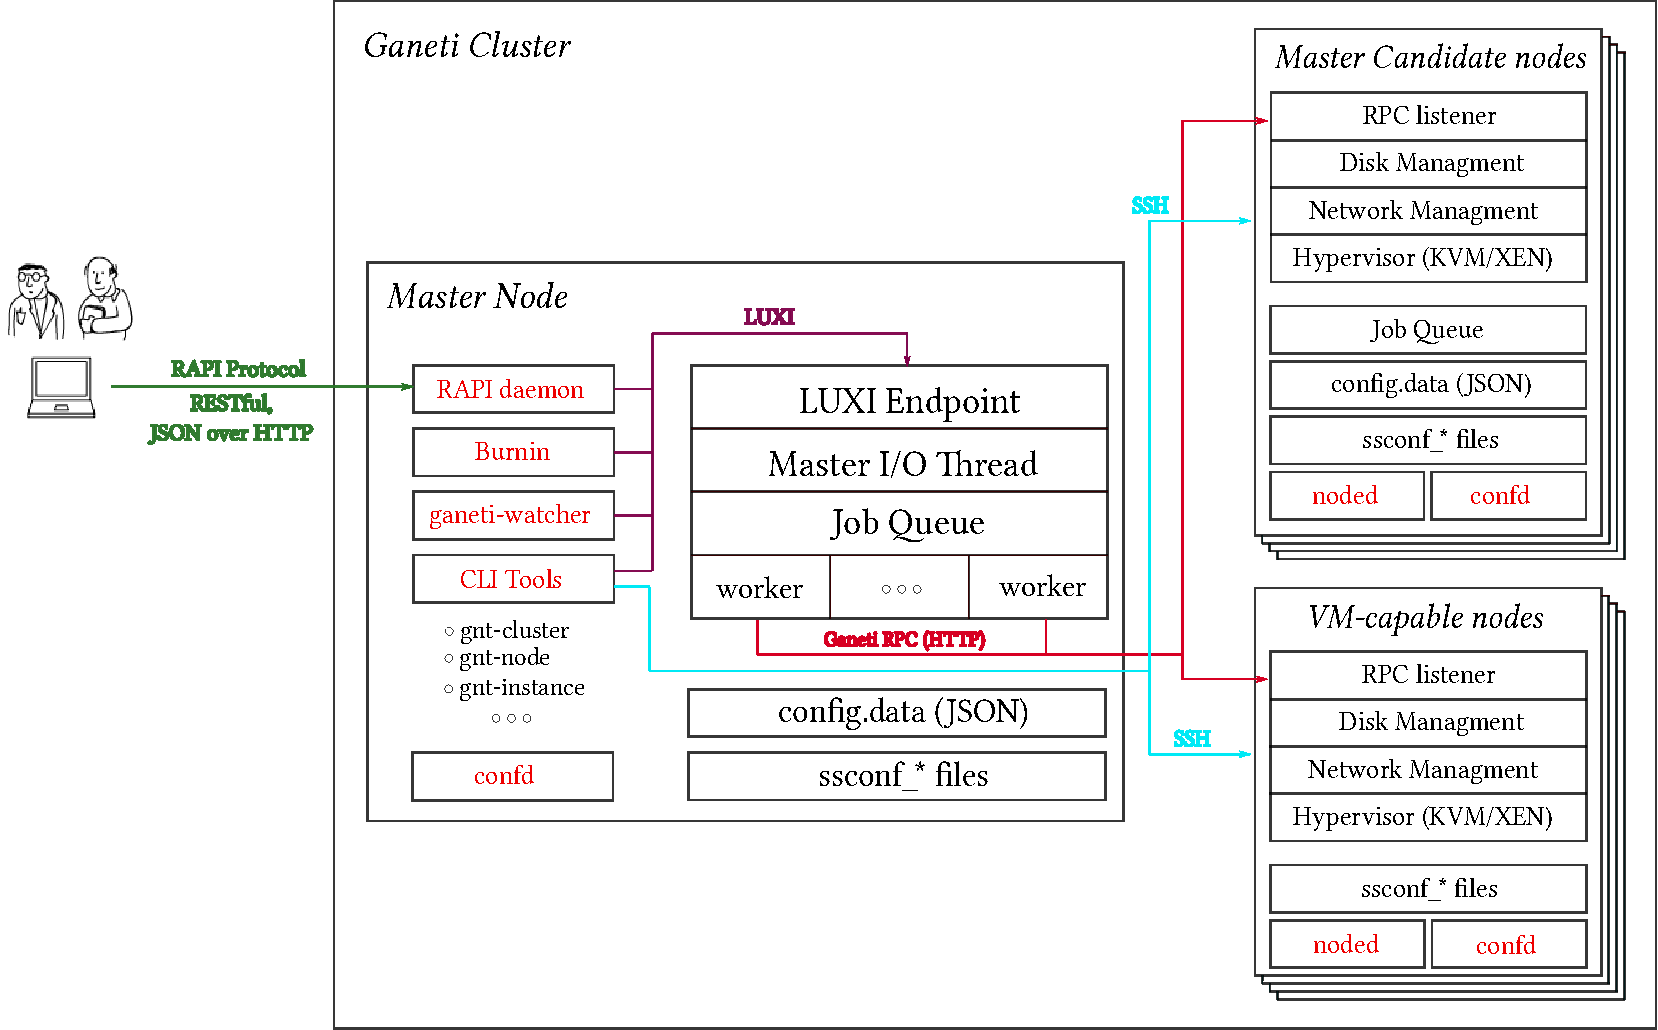
\includegraphics[width=1.0\maxwidth]{../figures/ganeti_arch_horizonal.pdf}
    \caption{Ganeti architecture, version 2.7.2\label{fig:gnt_arch}}
   \end{center}
\end{figure}

\emph{Nodes} are the basic cluster infrastructure in Ganeti. They serve
different roles and they can, and usually do, serve more than one. We could
group node roles into two major categories; The \emph{Administrative}
and the \emph{VM-capable} nodes. Nodes belonging in the first category, can
modify the cluster state, or take part in cluster related decisions like the
master node voting procedure. Nodes in second category can simply hosts
instances (VMs).

In more details, a node can belong in one, or more of the following roles:

\begin{description}
  \item[Master] \hfill \\
    It is the cluster coordinator node and it holds the authoritative copy of
    the cluster configuration. Every decision that could affect the cluster
    state managed by this node, because it is the only node which can execute
    commands. Only one master should exist every time in a Ganeti cluster.
  \item[Master Candidate] \hfill \\
    Nodes in this category have the full copy of the live cluster configuration
    and jobs. Only nodes belonging in this role can become master. This set of
    nodes called \emph{candidate pool}, and there is also a parameter called
    \texttt{candidate\_pool\_size}, which represents the number of candidates
    the cluster tries to maintain, automatically. Because the
    \texttt{candidate\_pool\_size} can have a huge impact in Ganeti performance,
    for reasons which we 'll explain later, it can be configured during
    initialization or modified via cluster related commands (\texttt{gnt-cluster
    *}).
  \item[Master Capable] \hfill \\
    Nodes in this category are not master candidates, but can become and
    promoted to master node, in cases when nodes in the candidate pool
    are less than the desired size. In such case, a randomly selected master
    capable node is promoted to master candidate. We could disable this flag
    and exclude some nodes from being master candidates in case when they have
    a less reliable hardware and we do not want to store sensitive information
    to them.
  \item[VM Capable] \hfill \\
    This is the default node state and means that the node can host instances.
    More specifically, the node will participate in instance allocation
    operations, capacity calculations, cluster checks, and other operations.
  \item[Offline] \hfill \\
    Nodes having this flag set have some special characteristics. They are still
    recorded in the Ganeti configuration, and can only take part in the
    master voting procedure, to ensure consistency. They are not allowed to
    become master. Enabling this flag to a master candidate node will demote
    it from candidate possibly, causing another node which is master capable to
    be promoted. Additionally, these nodes are not allowed to host primary
    instances. The main reason this role was added to Ganeti was to allow
    broken machines that are being repaired to remain in the cluster without
    introducing further problems.\\
  \item[Drained] \hfill \\
    Nodes in this state, will not participate in instance allocation operations,
    but all other operations as queries, or starting and stopping instances, are
    working without any restrictions. The actual intention is that nodes in this
    role have some issue and they are being evacuated for hardware repairs.
\end{description}

Previously, we made some references to Ganeti \emph{Cluster Configuration} and
\emph{Jobs} which are stored in the system as files. These files are stored
under the \texttt{/var/lib/ganeti} directory, and actually form a database for
the cluster. Every single piece of information that the cluster needs to operate
normally is stored in those files.

\subsection{Cluster Configuration}\label{subsec:config}

The cluster configuration is a set of files which are present in all, or a
subset of nodes depending on their usage. We could group them into three main
categories, namely:

\begin{description}
  \item[config.data] \hfill \\
  The cluster configuration database is a single JSON config file called
  \texttt{config.data}. The master node keeps a valid version of this file and
  it also replicates it to the master candidate nodes, for reliability
  reasons. Ganeti has a special way to handle \texttt{config.data} updates; It
  holds the \texttt{config.data} both in master memory and disk. The canonical
  version of the config exists at every moment in the master node memory, and
  the disk version will be updated from there. Every operation that updates a
  single object in the memory version of the \texttt{config.data}
  automatically causes a flush of the whole file to disk. If the config
  does not flushed successfully to disk, the operation will fail. The
  \texttt{config.data} file contains information about all the major Ganeti
  objects such as cluster, nodes, instances, networks, and their attributes.
  We will extensively talk about the \texttt{config.data} structure in the
  next chapters.

  \item[ssconf\_*] \hfill \\
  Besides the objects contained in the \texttt{config.data}, which change
  quite often, Ganeti also holds a set of configuration files which contain
  information that does not change frequently and needs to be present to all
  Ganeti nodes. These files are stored in the same directory as the
  \texttt{config.data} file and start with a \texttt{ssconf\_} prefix. For
  example, the ssconf file which contains the master IP value is called
  \texttt{ssconf\_master\_ip}, and so on. The main reason for the existence of
  the ssconf files is that the most frequent Ganeti operations should not need
  to contact the master node and overload him. In addition, we want some
  information to be accessible at every moment, even if the master node is
  down, so that we can use it from services external to the cluster, and
  avoiding the single point of failure that a master hard shutdown could
  introduce.

  \item[SSL certificates] \hfill \\
  Ganeti uses OpenSSL for encryption on the RPC layer, and SSH for executing
  commands. These SSL certificates are stored under the same directory as the
  rest of the configuration files and exist in all Ganeti nodes. The SSL
  certificates are automatically generated when the cluster is initialized, and
  are copied to the newly added nodes automatically along with the master's SSH
  host key. The cluster SSL key is stored in the \texttt{server.pem} file.
  There is a similar key for the RAPI daemon, the \texttt{rapi.pem} file. The
  \texttt{spice.pem} and \texttt{spice-ca.pem} files are used by SPICE
  connections to the KVM hypervisor, the \texttt{hmac.key} is used by the
  \texttt{ganeti-confd} daemon, the \texttt{cluster-domain-secret} file is used
  to sign information exchanged between separate clusters via a third party,
  and finally the Ganeti \texttt{known\_hosts} file are all the certificates
  maintained by Ganeti.
\end{description}

\subsection{Jobs}\label{subsec:jobs}

Jobs are the basic Ganeti operation, and the only way to modify the cluster's
state. They are stored as individual files in the file system, and serialized
using JSON format, which is the standard Ganeti serialization mechanism. A
job consists of one or more opcodes. That list of opcodes is processed
serially, and if an opcode fails, later opcodes are no longer processed and
the entire job will fail.

At any time, each job and each opcode can be, in a different status depending
on the stage of its execution. The job status is actually the status of its
first processed opcode. A complete status description follows:
\begin{description}
  \item[Queued] \hfill \\
    The job/opcode has been submitted, but has not been processed yet.
  \item[Waiting] \hfill \\
    The job/opcode is waiting for locks, or other factors, to proceed.
  \item[Running] \hfill \\
    The job/opcode is currently being executed.
  \item[Canceled] \hfill \\
    The job/opcode is waiting for locks, but is has been marked for
    cancellation by the user. It will never return to the \emph{Running}
    status.
  \item[Success] \hfill \\
    The job/opcode ran and finished successfully.
  \item[Error] \hfill \\
    The job/opcode has failed while executing, or the master daemon stopped
    before the job finishes its execution.
\end{description}

While job opcodes execute serially, jobs do not. Their execution order depends
on a variety of factors, apart from their incoming order, like their ability to
acquire all necessary locks, their priority, or probable dependencies with
other jobs. At any time, there are jobs that can be in one of the above
statuses. Similarly to the global cluster configuration files, jobs are stored
under a directory in the configuration path called \emph{queue}, which is
located by default under the \texttt{/var/lib/ganeti/queue} path.
The \emph{Job Queue} structure speeds
up operations because every job which is ready for execution can run
independently and so in parallel with the other jobs. In addition, storing
the jobs in a common folder makes it more convenient for the user to handle
and watch their progress, independently of Ganeti, and it also makes the
consistency checks that Ganeti does to the job list and jobs themselves a
simpler procedure. Queue structure also gives us the choice to prevent new
jobs from entering it by enabling the \emph{drained flag}. This is a feature
used mainly in cases when we have to make maintenance-related operations to
the cluster and we do not want any new incoming jobs affecting us.

Besides the regular jobs, the \emph{Job Queue} structure always contains three
more files, even if there are not any jobs running, pending, or canceled in
the cluster. Those are the \texttt{version} file, which denotes the queue
format version, the \texttt{lock} file, which is opened by the queue managing
process in exclusive mode, and the \texttt{serial} file, containing the last
job ID value used. Listing~\ref{lst:job_queue}, presents a high-level view of
the Ganeti Job Queue structure:

\includeminted[text]{../listings/job_queue.txt}{%
  Job Queue structure}{lst:job_queue}{frame=single}

In Listing~\ref{lst:job_structure}, we present the internal structure of a
randomly-selected job in Ganeti, with its most basic fields:

\includeminted[text]{../listings/job_structure.json}{%
  Job structure}{lst:job_structure}{linenos}

As we notice from this listing, a job consists of the \texttt{ops} field, short
for opcodes, the job \texttt{id}, and three \texttt{timestamp} fields that
indicate when the job passed from the various statuses we presented earlier.
This job, consists of an opcode list with a single element, and
represents an instance create operation as indicated by the \texttt{OP\_ID}
field, i.e, \texttt{OP\_INSTANCE\_CREATE}. Every opcode also has its own
timestamps, as the job, so that the user can be informed with more details
about the exact time every single opcode passed from the various statuses.
The rest fields presented, are related to the specific opcode, to make the
reader better understand how Ganeti stores and handles the parameters we
give in a commonly used job like the creation of an instance. These are
the iallocator algorithm, the hypervisor chosen, and the opportunistic
locking choice for the lock retrieval, a topic that we 'll cover later in
Section~\ref{subsec:locks}.

Besides the above fields, we distinguish two important fields that will help
us to better understand how a job executes by the Ganeti processor; the
\texttt{priority} and \texttt{depends} fields.

The job \texttt{priority} is an integer number; the lower the number the
higher the opcode's priority is. This is a very helpful attribute in job
queue handling, because in cases we want to run a job like an emergency
shutdown as soon as possible, we want to overcome factors that could
delay us. The priority range is [-20..19], and jobs submitted without
priority assigned the default zero value. To avoid starvation, a job can
change its own priority after a certain amount of retries, or a certain
amount of time. One interesting thing is that opcodes also have their own
priorities. So, the job priority is the same as its first unprocessed opcode.
This behavior, combined with the fact that the job processor returns the job
back to the queue after each opcode completion, means that if there are opcodes
of higher priority submitted in the meantime of a job execution, these will
first try to acquire their locks and as result the job that was
\texttt{Running} will go to the \texttt{Waiting} status again. That behavior
makes the job queue structure a lot more versatile.

The \texttt{depends} field of a job, is an optional property which defines
dependencies on other jobs. Clients can submit jobs in the right
order and proceed to wait for changes made to them. The master daemon will
take care of everything, Section~\ref{subsec:daemons} covers that topic. Jobs
waiting for dependencies are in the \texttt{Waiting} status. In Listing
\ref{lst:job_deps}, we present a simple example of job dependencies:

\includeminted[text]{../listings/job_deps.txt}{%
  Job dependency diagram}{lst:job_deps}{frame=single}

The job queue must be consistent between the master node and the master
candidates, just like the cluster configuration files. Failures to replicate a
job to other nodes will be only flagged as error in the master daemon log if
more than half of nodes fail to copy it, otherwise the failure will be ignored
and the operation will continue normally. This relies on the fact that the
next update for already running jobs, will retry the update.

Now we will present the job execution procedure from a high-level view; the
\emph{``Life of a Ganeti job"}, from the time the user submits it till its
completion:

\begin{enumerate}
  \item Client submits the job. The appropriate opcode or a list of opcodes
        if the job consists of multiple opcodes, will be built in the client
        side. The opcode contains all the available information that Ganeti
        needs to execute the operation. For example, an
        \emph{OpInstanceCreate} opcode contains the name of the instance,
        the os\_type, the hypervisor, or instance-related parameters such as
        the beparams, the hvparams, the nicparams, and so on.
  \item Then the list of the opcode\{s\} will be sent via the LUXI protocol
        in the master daemon, who will generate a new job identifier depending
        on the value of the serial file, and it will assign it to the job.
        Then the master daemon writes the job to his local disk and replicates
        it to the master candidates. The job must be copied successfully at half
        of the candidates at least, otherwise the operation will fail. Then,
        the identifier is returned to the client using the LUXI protocol again.
  \item After the job\_id is returned to the client, the master daemon builds
        the job object named \texttt{\_QueuedJob}, and adds a new task to
        the workerpool. The task is the job object and the workerpool is a
        heap queue. The tasks are ordered in the heap queue in respect to
        the job's priority primarily, and if the priorities match, to an
        increasing number which denotes their incoming order.
  \item As soon as a new task is added to the heap queue, a pool of job queue
        workers with currently 25 threads will be notified for new arrivals.
        Those threads wait for new jobs to arrive. If all threads
        are busy, the job will have to wait until one of them become
        available. The first worker finishing its work will grab it.
        Otherwise one of the waiting threads will pick up the new job.
  \item When a job assigned to a worker it is time for the job to start its
        execution. The worker does not know nothing about the opcodes that
        the job contains. He just passes the opcode to the Ganeti's
        processor who dispatches them to the appropriate Logical Units,
        the \emph{LUs} in short. There is a Logical Unit for each Ganeti
        opcode which knows how to deal with it. The LU is the part of Ganeti
        which finally executes the operation which will modify the
        cluster's state. The rest responsibilities of a worker thread include
        the appropriate handling of the job queue lock, the notification of
        other threads when it finishes its work, and generally taking care of
        the job's smooth execution.
  \item If the user chooses to wait for job status updates and does not make
        use of the \texttt{--submit} flag, he waits by calling a waiting RPC
        function. The mechanism underlying the waiting function is an
        inotify manager who responds to events happen in the job file
        located to disk. In this case, log messages may be shown to the user
        depending on the job. The user can also cancel the job while it is
        waiting in the queue.
  \item The client can also archive the job, which then moved to a history
        directory called \emph{archive} ,i.e., the default path is the
        \texttt{/var/lib/ganeti/queue/archive} directory. This can be done in
        order to speed up the queue handling, because by default, jobs in the
        archive directory do not touched by any function.
\end{enumerate}

\subsection{Ganeti Daemons}\label{subsec:daemons}

We have already made a few references to the Ganeti daemons in previous
sections. Now we will talk in more details about the internal structure of
Ganeti, and particularly the set of daemons that it is divided into. Ganeti
consists of a growing number of daemons. Each of these deals with a specific
task that the cluster has to face, and communicates with the rest using a
variety of protocols. Specifically, as of Ganeti version 2.7, we have four
daemons. The situation is as follows:

\begin{description}
  \item[Master Daemon] \hfill \\
    The master daemon runs on a single node only, the master node. Currently is
    written in python and deals with every cluster operation. It is the Ganeti's
    heart because it is responsible for the overall cluster coordination.
    Without it, no modification can be performed on the cluster. This is the reason
    why it is the most heavy loaded daemon of all. It receives the commands
    given by the clients, either through the Command Line
    tools or the Remote API, parses them, and executes the appropriate
    operation. Creates, and manages the jobs that will execute those commands,
    handles the locks, and ensures that race conditions will never occur. It is
    also responsible for managing, and maintaining the cluster configuration files,
    updating them when it is necessary, and replicating them to the master
    candidates, in addition to the job queue. Each job is managed by a separate
    python thread. The basic python threads which managed by the master daemon
    are presented below:

    \begin{itemize}
      \item \emph{The main I/O thread}: It is a single thread. The
            \texttt{masterd} is build around this thread. It accepts connections
            in the master socket and setups/shutdowns the other thread pools.
      \item \emph{The job queue worker threads}: This pool consists of 25
            threads, each of which executes the jobs submitted by the clients.
            They are long-lived threads and are initialized during the daemon
            startup.
      \item \emph{The client worker threads}: The client worker pool contains 16
            threads. They handle the connections in the master socket, one thread
            per connected socket, parse LUXI requests, and send data back to the
            clients. They are also being built during daemon startup.
      \item \emph{The RPC worker threads}: This is not actually a pool like the
            above two categories. The thread size depends on the RPC call;
            single-node or multi-node. They interact with nodes using HTTP based
            RPC calls.
    \end{itemize}

    The \texttt{masterd} keeps some interaction paths for the communication with
    the rest Ganeti daemons. More specific, the interaction between the Command
    Line tools which are located in the master node, and the RAPI daemon is done
    with a custom protocol called LUXI. LUXI is a UNIX-socket based protocol of
    JSON-encoded messages. The UNIX socket permissions itself will determine the
    access rights. The LUXI API allows both job related operations, and cluster
    query functions.

    The communication between the master daemon and the rest node daemons is
    done through RPC calls, using HTTP\{S\} simple PUT/GET of JSON-encoded
    messages. Communication between master and nodes is protected using SSL/TLS
    encryption. Both the clients and the server must have the cluster-wide
    shared SSL/TLS certificate, and verify it when establishing the connection
    by comparing fingerprints. For highly-traffic commands like image dumps, or
    low level commands such as restarting the \texttt{node-daemon}, a simple SSH
    protocol is used. The master node must share the cluster-wide shared SSH key
    with the rest nodes of the cluster.

    During startup, the \texttt{masterd} will confirm in coordination with the
    node daemons that the node it is running, is the master node of the cluster,
    indeed. This is done via a voting procedure where all the nodes take part,
    even the offline ones. For successful confirmation the \texttt{masterd} has
    to get half plus one positive answers. When the \texttt{masterd} receives a
    SIGINT or SIGTERM signal, it stops accepting new jobs, and prepares to shut
    down as soon as the jobs that are currently running finish their execution.
    At the meanwhile, it still answers to LUXI
    requests. Pending jobs are re-added to the queue in \texttt{Queued} state
    after the daemon restarts. If a hard shutdown requested the cluster may be
    leaved in an inconsistent state.

    The current Ganeti daemon structure suffers from many performance problems
    caused by the various protocols involved in interaction between daemons, and
    by the many python threads that are created which increase lock contention,
    log pollution and memory usage. This is the reason why from version 2.9,
    Ganeti daemon subdivision will change to improve the current situation.
  \item[Node Daemon] \hfill \\
    The \texttt{noded} runs on all the nodes of a cluster. It is also written in
    python, and it is responsible for receiving the requests made by the
    \texttt{masterd} over RPC, and executes them using the appropriate backend
    tool ,e.g., hypervisors, DRBD, LVM. It executes almost all operations that
    modify the node's state, like creating disks for instances, activating disks,
    starting/stopping an instance and so on. If a \texttt{noded} stops, the
    \texttt{masterd} will not be able to talk to this daemon, but the instances
    will not be affected.
  \item[Rapi Daemon] \hfill \\
    The \texttt{rapid} is written in python, and runs automatically on the master
    node only. By default, listens on TCP port 5080 and uses SSL/TLS encryption.
    Both those parameters can change via command line. Ganeti supports a Remote
    API protocol which is JSON over HTTP, designed over the REST principle, for
    enabling communication with external clients, to easily retrieve information
    about the cluster state or modifying it. The \texttt{ganeti-rapid} waits for
    requests issued remotely through that protocol. Then, it forwards them via
    the LUXI protocol to the master daemon to deal with them.

    \texttt{Rapid} reads its users and their rights from a file on startup,
    which is usually located under the \texttt{/var/lib/ganeti/rapi/users} path.
    Changes to that file will be loaded automatically. Most query operations
    are allowed without authentication. Modification operations though, require
    authentication in order to be executed.
  \item[Configuration Daemon] \hfill \\
    The configuration daemon is written in Haskell and runs on all master
    candidate nodes, since the configuration exists only on that group of nodes.
    This daemon is used to answer queries related to the configuration of a
    cluster. It makes sure that we have a highly-available and very fast way to
    query cluster configuration values. The \texttt{config.data} is reloaded
    automatically from disk every time it is updated. The requests are made
    through an HMAC authenticated JSON-encoded custom protocol over UDP, and
    meant to be used by parallel querying all the master candidates, or a
    subset of them, getting the most up to date answer by comparing the
    value of the \texttt{config.data}'s serial number, named \texttt{serial\_no}.
    The queries are answered from a cached copy of the config which it keeps in
    memory, so no disk space is required in order to get an answer. Queries are
    also contain a ``salt" which they expect the answers to be sent with, and
    clients are supposed to accept only answers which contain salt generated by
    them. The configuration daemon answers simple queries such as:

    \begin{itemize}
      \item master node
      \item master candidate, offline nodes
      \item instance list, primary nodes
      \item cluster info
      \item job list, and more
    \end{itemize}

    In Ganeti 2.7 we can also disable the \texttt{confd} during build time
    using the \texttt{--disable-confd} flag, if it is not needed in our setup.
    The \texttt{confd} serves both network-oriented queries about the static
    configuration, and local UNIX socket queries about the current status of the
    system including live data configuration. To answer queries of the second
    category the daemon has to communicate with the node daemons through RPC
    calls. In next Ganeti versions, it is intended those two functionalities to
    be separated into two different daemons, for simplicity and security
    reasons.
\end{description}

Finally, we have to mention that there exists a log file per daemon model, which
are by default stored under \texttt{/var/log/ganeti} directory. Those log files
are:

\begin{itemize}
  \item The master-daemon.log, for the MasterD.
  \item The node-daemon.log, for the NodeD.
  \item The rapi-daemon.log, for the RapiD.
  \item The conf-daemon.log, for the ConfD.
\end{itemize}

\subsection{Ganeti Locking}\label{subsec:locks}

We have already covered the most major Ganeti parts. The last, but not least,
part we will cover is the Ganeti \emph{Locking} library and the way it is
implemented. Locking libraries are vital for every project, affecting the overall
performance. They must preserve data coherency, prevent deadlocks and thread/job
starvation. Ganeti Locking library has passed through many stages but still
improves and extends its features. In earlier Ganeti versions (\emph{1.x}),
there was a single global cluster lock for most operations, which made
inevitable the execution of parallel operations. In Ganeti \emph{v2.0} a
complete redesign of the locking library has been made, which allowed the
parallel execution of multiple operations. The locking library was also
drastically improved in version \emph{v2.1}, but the last major change was made
in \emph{v2.3} when the job priorities was firstly introduced. A feature called
\emph{Opportunistic Locking} was added lately, at \emph{v2.7}, which also
improved the parallel execution of some operations, mainly the instance
creations. Below we will present the current Ganeti Locking library and how
it is working \emph{``under the hood"}.

\begin{description}
  \item[The Locks] \hfill \\
    Locks are represented by objects of \texttt{locking.SharedLock} class. These
    locks are declared by the Logical Units located in the \texttt{cmdlib.py}
    module, and are acquired by the Processor which is found in the
    \texttt{mcpu.py} module, with the aid of the Ganeti Locking library, in
    \texttt{locking.py}. There are several locking levels which must acquired in
    specific order. These levels are the following:

    \begin{enumerate}
      \item Cluster level or BGL from Big Ganeti Lock.
      \item Instance level.
      \item Node allocation level or NAL.
      \item Nodegroup level.
      \item Node level.
      \item Node resource level.
      \item Network level.
    \end{enumerate}

    These locks must be acquired in an increasing order. Each lock has the
    following possible statuses:

    \begin{itemize}
      \item \emph{Unlocked}, anyone can grab the lock.
      \item \emph{Shared}, anyone can grab the lock but in shared mode only.
      \item \emph{Exclusive}, only one can hold the lock.
    \end{itemize}

    Besides the order in which the locks acquired, there are some extra rules
    which must be preserved:

    \begin{itemize}
      \item \emph{Cluster level}, resides the Big Ganeti Lock, or BGL. It is the
        first lock which must be acquired before performing any operation in the
        cluster. Can be acquired either in shared or exclusive mode, but
        acquiring it in exclusive mode is discouraged and should be avoided.
      \item \emph{Instance level}, resides the instance locks. They have the
        same name as the instances they protect, and are created when a new
        instance is added to the cluster. They are acquired as set, which means
        that if we need more than one instance locks we must acquire them at the
        same time. Internally the locking library acquire them in alphabetical
        order.
      \item \emph{Node level}, resides the node locks and have the same names as
        the nodes they protect. They are also
        acquired as a set, and internally acquired in alphabetical order. We
        should first acquire all the instance level locks that reside in a node,
        before we acquire the node lock itself. Ofcourse, before the node locks,
        we should already have the BGL acquired, preferably in shared mode.
      \item \emph{Node Resource level}, it is used for node resources protection,
        as it name reveals, and should be used by operations with possibly high
        impact on the node's disks.
      \item \emph{Node Allocation level}, this lock is similar to the BGL in the
        sense that it has its own level and there is only one. It must be acquired
        after the instance locks and before the nodegroup locks, and used for
        instance allocation related operations. As a rule-of-thumb, NAL must be
        acquired in the same mode as the node and/or the node-resource locks. It
        blocks instance allocations for the whole cluster and can be acquired
        either in shared or exclusive mode. OpCodes doing instance allocations should
        acquire it in exclusive mode. When an Opcode blocks all or a significant
        amount of the cluster's locks, it should be acquired in shared mode. The
        NAL lock should be released when the set of acquired locks for an opcode
        reduces to the working set, to allow allocations to proceed.
    \end{itemize}

    Besides the above levels, we also have the \texttt{ConfigWriter} lock which is
    shared among those functions that read the \texttt{config.data} file, and
    acquired exclusively by functions that modifying it. This extra lock level allows
    the \texttt{config.data} replication to the master candidate nodes using the
    \texttt{rpc.call\_upload\_file} call, without holding the node level locks since
    the RPC function caller already holds the config lock in exclusive mode. This
    have the advantage that the config distribution can run in parallel with other
    cluster operations.

    Similarly to the \texttt{ConfigWriter} lock, exists the Big \emph{Job Queue}
    lock. It is used from all classes involved in the queue handling. Job queue
    functions acquiring it can be safely called from the rest of the code,
    because the lock is released before leaving the job queue again, something
    that prevents deadlocks. Unlocked queue functions must only be called from
    those functions, which have already acquired the lock beforehand.

  \item[Ganeti Locking Library] \hfill \\
    As we have already mentioned, locks in Ganeti are represented by objects.
    The basic class which implements a lock in Ganeti is the \texttt{SharedLock}
    class located in the \texttt{locking.py} module. All locks needed in the
    same level must be acquired together. So, a class is needed to take care of
    acquiring the locks always in the same order, thus preventing deadlocks.
    This class is the \texttt{locking.LockSet} class, a container of one or more
    \texttt{SharedLock} instances, which provides an interface to add/remove
    locks, to acquire, and subsequently release any number of those locks
    contained in it, distinguished by name. As this class is beyond the scope of
    this document, we will not present it further. In this section we will
    focus in the \texttt{SharedLock} class, to understand the Ganeti's approach
    to its locking requirements.

    \texttt{SharedLock} class implements a shared lock. Multiple threads can
    acquire the lock by calling \texttt{acquire(shared=1)}. Exclusive acquirers
    should call \texttt{acquire(shared=0)}. Since Ganeti first introduced job
    priorities in \emph{v2.3}, the internal structure of \texttt{SharedLock}
    class also changed to support them. All pending acquires for a lock with
    different priorities is contained in a heap queue similar to the worker pool
    structure, named \texttt{\_\_pending}. The heap queue does automatic sorting,
    automatically taking care of priorities. For each priority there is a single
    plain list ([]) of pending acquires. This is a normal in-order list of
    conditions~\footnote{A condition variable in Ganeti is a bit different from
    the Python's built-in \texttt{threading.Condition} class. It uses POSIX pipes
    in addition to the operating system support on timeouts on file descriptors
    (see \texttt{select(2)}). All clients of the condition use \texttt{select} or
    \texttt{poll} to wait for notifications. In a higher level-of-view a condition
    variable has \texttt{acquire()} and \texttt{release()} methods that call the
    associate lock methods. Also has a \texttt{wait()}, \texttt{notify()} and
    \texttt{notifyAll()} methods. Threads waiting for a particular change of state
    call \texttt{wait()} repeatedly until they see the desired state. Threads that
    modify the state will call \texttt{notify()} or \texttt{notifyAll()} when they
    change the state in a desired way for the waiting threads.} to be notified
    when the lock can be acquired. Shared acquires are grouped together by
    priority and the condition for them is stored in a separate dictionary
    of shared acquires called \texttt{\_\_pending\_shared}. There is also a
    dictionary called \texttt{\_\_pending\_by\_prio} which keeps references for
    the per-priority queues indexed by priority for faster access.

    When the lock is released, the code locates the list of pending acquires
    with the highest priority waiting. Due to the heap queue behavior, this is
    the first element in the structure. The first, zero indexed condition of the
    list is notified. Once all waiting threads receive the
    notification, the condition is removed from the list, the code processes the
    second condition and so on. When the list of conditions is empty it is
    removed from the list, and the list of conditions of the second priority in
    the heap is processed. In
    Listing~\ref{lst:lock_queue}, we present a possible state of the internal
    queue from a high-level view. Conditions are shown as waiting threads.
    Assuming we have no timeouts or other modifications, for simplicity reasons,
    the lock will be acquired by the threads in the following order (concurrent
    acquirers in parenthesis):

    thread-Ex1, thread-Ex2, (thread-Sh1/thread-Sh2/thread-Sh3),
    (thread-Sh4/thread-Sh5), thread-Ex3, thread-Sh6, thread-Ex4, thread-Ex5

    \includeminted[text]{../listings/lock_queue.txt}{%
      Structure of the \texttt{SharedLock} class}{lst:lock_queue}{}

  \item[Locking Granularity] \hfill \\
    With the current locking policy, each Logical Unit acquires/releases the
    locks it needs; this means that locking is at the Logical Unit level.
    Ofcourse, each LU has its own locking requirements. Logical Units declare
    their locks and then execute their code with the appropriate locks held. In
    Listing~\ref{lst:lock_order}, we present how the Ganeti Processor with the
    aid of the Logical Units executes an OpCode from an abstracted point of
    view, which pays more attention to the lock handling.
  \item[Opportunistic Locking] \hfill \\
    The last major change in Ganeti locking library was made in \empty{v2.7},
    when firstly introduced the \emph{Opportunistic Locking} feature. The
    motivation behind this change was the need of more instance creations in a
    shorter amount of time. As of Ganeti \emph{v2.6}, instance creations acquire
    all locks when an iallocator algorithm was used, causing a lot of lock
    congestion on node locks when someone tried to create many instances at
    once. This situation can become worse when we are waiting for DRBD
    synchronization between disks, if we choose the \texttt{drbd} template for
    an instance. As a result, even on big clusters with multiple nodegroups all
    instance creations were serialized. The main objective was to speed up
    instance creations in combination with an iallocator even when the cluster's
    balance is sacrificed in the process. The cluster can be rebalanced latterly,
    by using external Ganeti tools ,e.g., \texttt{hbal}. So, the opportunistic
    locking reduces the number of node locks acquired for instance creations,
    causing many creation operations to run in parallel. More specific, instead
    of forcibly acquiring all node locks for creating an instance using an
    iallocator, only those locks available will be acquired, and the iallocator
    algorithm will run on those nodes we have succeeded to acquire their locks.
\end{description}

\includeminted[text]{../listings/lock_order.py}{%
  \text{OpCode} execution path}{lst:lock_order}{linenos}
